\documentclass[11pt]{article}
\usepackage[table]{xcolor}
\usepackage{style/acl2017}
\usepackage{times}
\usepackage{fixfoot}

\usepackage{amsmath}
\usepackage{amssymb}
\usepackage{graphicx}
\usepackage{xspace}
\usepackage{url}
\usepackage{bm}

\aclfinalcopy
\def\aclpaperid{516}


\newcommand{\apriori}{\textit{a priori} }
\newcommand{\aposteriori}{\textit{a posteriori} }
\newcommand{\map}{\textit{maximum a posteriori} }

\newcommand{\g}{\, | \,}

\newcommand{\argmax}{\operatornamewithlimits{argmax}}
\newcommand{\argmin}{\operatornamewithlimits{argmin}}

\newcommand{\ndim}[1]{#1\nobreakdash\discretionary{-}{-}{-}\hspace{0pt}dimensional}

\newcommand{\dquote}[1]{\textquotedblleft#1\textquotedblright}
\newcommand{\squote}[1]{\textquoteleft#1\textquoteright}
\newcommand{\abr}[1]{\textsc{#1}\xspace}
\newcommand{\twentynews}{\textsc{20news}}
\newcommand{\hidetext}[1]{}

\definecolor{byublue}{HTML}{00305E}
\definecolor{byublue2}{HTML}{114477}
\definecolor{byublue3}{HTML}{336699}
\definecolor{byublue4}{HTML}{628CB6}
\definecolor{byublue5}{HTML}{91B2D2}
\definecolor{byublue6}{HTML}{ABC8E4}
\definecolor{byublue7}{HTML}{D1E4F6}
\definecolor{byutan}{HTML}{C5AF7D}
\definecolor{byured}{HTML}{990011}
\definecolor{byugreen}{HTML}{007722}
\definecolor{byugreen2}{HTML}{CCEDCE}
\definecolor{byuorange}{HTML}{EE8800}

                                        
\newcommand{\comment}[2]{\colorbox{cyan}{\parbox{.8\linewidth}{#1:#2}}}

\newcommand{\jbgcomment}[1]{  \colorbox{red}{   \parbox{.8\linewidth}{ JBG: #1}  }}

\newcommand{\anch}[1]{\mathcal{G}_{#1}}
\newcommand{\pword}[1]{\mathit{g}_{#1}}

\DeclareFixedFootnote{\statsigoracle}{Significant at $p<0.01/4$ under
  two-tailed $t$-tests with a Bonferroni correction.  For each
  evaluation, we verify the normality~\cite{scipy-normaltest} and use
  two-tailed $t$-tests with Bonferroni correction to determine whether
  the differences between methods are significant.}

\DeclareFixedFootnote{\statsiguser}{Significant at $p<0.01$ when using
  Wilcoxon's signed-rank test.}

\newcommand{\filename}[1]{2017_acl_multiword_anchors/#1}
\addtolength\titlebox{.2in}

\title{Tandem Anchoring: \\ A Multiword Anchor Approach for Interactive Topic Modeling}

\author{Jeffrey Lund, Connor Cook, Kevin Seppi \\
        Computer Science Department \\
        Brigham Young University \\
        \{jefflund,cojoco,kseppi\}@byu.edu
        \And
        Jordan Boyd-Graber \\
        Computer Science Department \\
        University of Colorado Boulder \\
        jordan.boyd.graber@colorado.edu}

\date{}

\begin{document}

\maketitle

\begin{abstract}
Interactive topic models are powerful tools for understanding
large collections of text.
However, existing sampling-based interactive topic modeling approaches
scale poorly to large data sets.
Anchor methods, which use a single word to uniquely identify a topic,
offer the speed needed for interactive work but lack both
a mechanism to
inject prior knowledge and lack the intuitive semantics needed for user-facing
applications.
We propose combinations of words as anchors, going beyond
existing single word anchor algorithms---an approach we call ``Tandem
Anchors''.
We begin with a synthetic investigation of this approach
then apply the approach to interactive topic modeling in a user
study and compare it to interactive and non-interactive approaches.
Tandem anchors are faster and more intuitive than existing interactive approaches.

\end{abstract}

\section*{}
\label{sec:intro}

Topic models distill large collections of text into topics,
giving a high-level summary of the thematic structure of the data without
manual annotation.
In addition to facilitating discovery of topical
trends~\cite{topical-guide}, topic modeling is used for a wide
variety of problems including
document classification~\cite{topic-classification},
information retrieval~\cite{lda-ir},
author identification~\cite{author-topic},
and sentiment analysis~\cite{topic-sentiment}.
However, the most compelling use of topic models is to help users understand
large datasets~\cite{termite}.

Interactive topic modeling~\cite{hu-14:itm} allows non-experts to refine
automatically generated topics, making topic models less of a ``take it or
leave it'' proposition.
Including humans input during training improves the quality of the
model and allows users to guide topics in a specific way, custom
tailoring the model for a specific downstream task or
analysis.

The downside is that interactive topic modeling is slow---algorithms typically
scale with the size of the corpus---and requires non-intuitive information from
the user in the form of must-link and cannot-link
constraints~\cite{andrzejewski-09}.
We address these shortcomings of interactive topic modeling by using an
interactive version of the \emph{anchor words} algorithm for topic models.

The anchor algorithm~\cite{anchors-practical} is an alternative topic modeling
algorithm which scales with the number of
unique word types in the data rather than the number of documents or tokens
(Section~\ref{sec:vanilla-algo}).
This makes the anchor algorithm fast enough for interactive use, even in
web-scale document collections.

A drawback of the anchor method is that anchor words---words that have high
probability of being in a \emph{single} topic---are not intuitive.
We extend the anchor algorithm to use multiple anchor words in tandem (Section
\ref{sec:multiword-extension}).
Tandem anchors not only improve interactive refinement, but also make the
underlying anchor-based method more intuitive.

For interactive topic modeling,
tandem anchors produce higher quality topics than single word anchors
(Section~\ref{sec:oraclular-experiments}).
Tandem anchors provide a framework for fast interactive topic modeling: users
improve and refine an existing model through multiword anchors
(Section~\ref{sec:interactive-experiments}).
Compared to existing methods such as Interactive Topic Models~\cite{hu-14:itm},
our method is much faster.

\section{Vanilla Anchor Algorithm}
\label{sec:vanilla-algo}

The anchor algorithm computes the topic matrix $\bm{A}$,
where $\bm{A}_{v,k}$ is the conditional probability of observing word $v$ given
topic $k$, e.g., the probability of seeing the word ``lens'' given the
\underline{camera} topic in a corpus of Amazon product reviews.
\newcite{nmf-provably} find these probabilities by assuming that every topic
contains at least one `anchor' word which has a non-zero probability only in
that topic.
Anchor words make computing the topic matrix $\bm{A}$ tractable because the
occurrence pattern of the anchor word mirrors the occurrence pattern of the
topic itself.

To recover the topic matrix $\bm{A}$ using anchor words, we first compute a $V
\times V$ cooccurrence matrix $\bm{Q}$, where $\bm{Q}_{i,j}$ is the conditional
probability $p(w_j \g w_i)$ of seeing word type $w_j$ after having seen $w_i$ in the
same document.
A form of the Gram-Schmidt process on $\bm{Q}$ finds anchor words $\{g_1 \dots
g_k\}$~\cite{anchors-practical}.

Once we have the set of anchor words, we can compute the probability of a topic
given a word (the inverse of the conditioning in $\bm{A}$).
This coefficient matrix $\bm{C}$ is defined row-wise for each word~$i$
\begin{equation}
\bm{C}^*_{i,\cdot} = \argmin_{C_{i,\cdot}} D_{KL} \left( \bm{Q}_{i,\cdot} \bigg\| \sum_{k=1}^K \bm{C}_{i,k} \bm{Q}_{g_k,\cdot} \right),
\label{eq:solve-c}
\end{equation}
which gives the best reconstruction (based on \mbox{Kullback-–Leibler}
divergence $D_{KL}$) of non-anchor words given anchor words' conditional probabilities.
For example, in our product review data, a word such as ``battery'' is a convex combination of the anchor words' contexts ($
\bm{Q}_{g_k,\cdot}$) such as ``camera'', ``phone'', and ``car''.
Solving each row of $C$ is fast and is embarrassingly parallel.
Finally, we apply Bayes' rule to recover the topic matrix $\bm{A}$ from the
coefficient matrix $\bm{C}$.

The anchor algorithm can be orders of magnitude faster
than probabilistic inference~\cite{anchors-practical}.
The construction of $\bm{Q}$ has a runtime of $O(D N^2)$ where $D$ is the
number of documents and $N$ is the average number of tokens per document.
This computation requires only a single pass over the data and can
be pre-computed for interactive use-cases.
Once $\bm{Q}$ is constructed, topic recovery requires $O(K V^2 + K^2 V I)$,
where $K$ is the number of topics, $V$ is the vocabulary size, and $I$ is the
average number of iterations (typically 100--1000).
In contrast, traditional topic model inference typically
requires multiple passes over the entire data.
Techniques such as Online \textsc{lda}~\cite{online-lda} or Stochastic Variation
Inference~\cite{stochastic-variational} improves this to a single
pass over the entire data.
However, from Heaps' law~\cite{heaps-law} it follows that $V^2 \ll D N$ for large datasets,
leading to much faster inference times for anchor methods compared to
probabilistic topic modeling.
Further, even if online inference could incorporate human guidance, a
single pass takes too long for interactive use.

\section{Tandem Anchor Extension}
\label{sec:multiword-extension}

\begin{table}
\begin{center}
\small
\begin{tabular}{p{.1\textwidth} p{.35\textwidth}}
\hline\hline
Anchor   & Top Words in Topics\\\hline
backpack & backpack camera lens bag room carry fit cameras equipment comfortable\\
camera   & camera lens pictures canon digital lenses batteries filter mm photos\\
bag      & bag camera diaper lens bags genie smell room diapers odor\\\hline
\end{tabular}
\end{center}
\caption{Three separate attempts to construct a topic concerning camera bags in
Amazon product reviews with single word anchors.
This example is drawn from preliminary experiments with an author as the user.
The term ``backpack'' is a
good anchor because it uniquely identifies the topic. However,
both ``camera'' and ``bag'' are poor anchors for this topic.}
\label{tab:camera}
\end{table}

Single word anchors can be opaque to users.
For an example of bewildering anchor words, consider a \underline{camera bag}
topic from a collection of Amazon product reviews (Table~\ref{tab:camera}).
The anchor word ``backpack'' may seem strange.
However, this dataset contains nothing about regular backpacks; thus, ``backpack'' is unique to \underline{camera bags}.
Bizarre, low-to-mid frequency words are often anchors because anchor words must
be \emph{unique} to a topic;
intuitive or high-frequency words cannot be anchors if they have
probability in \emph{any other topic}.

The anchor selection strategy can mitigate this problem to some degree.
For example, rather than selecting anchors using an approximate convex hull in
high-dimensional space, we can find an exact convex hull in a low-dimensional
embedding~\cite{anchors-tsne}.
This strategy will produce more salient topics but still makes it difficult
for users to manually choose unique anchor words for interactive topic
modeling.

If we instead ask users to give us representative words for this topic, we
would expect combinations of words like ``camera'' and ``bag.''
However, with single word anchors we must choose a single word to anchor each
topic.
Unfortunately, because these words might appear in multiple topics,
individually they are not suitable as anchor words.
The anchor word ``camera'' generates a general camera topic instead of camera
bags, and the topic anchored by ``bag'' includes bags for diaper
pails (Table~\ref{tab:camera}).

Instead, we need to use sets of representative terms as an interpretable,
parsimonious description of a topic.
This section discusses strategies to build anchors from multiple words and
the implications of using multiword anchors to recover topics.
This extension not only makes anchors more interpretable but also
enables users to manually construct effective anchors in interactive
topic modeling settings.

\subsection{Anchor Facets}

We first need to turn words into an anchor.
If we interpret the anchor algorithm geometrically, each row of $\bm{Q}$
represents a word as a point in $V$-dimensional space.
We then model each point as a convex
combination of anchor words to
reconstruct the topic matrix $\bf{A}$ (Equation~\ref{eq:solve-c}).
Instead of individual anchor words (one anchor word per topic), we use anchor
{\bf facets}, or sets of words that describe a topic.
The facets for each anchor form a new {\bf pseudoword},
or an invented point in $V$-dimensional space
(described in more detail in Section~\ref{sec:combine-facets}).

While these new points do not correspond to words in the vocabulary,
we can express non-anchor words as convex combinations of
pseudowords.
To construct these pseudowords from their facets, we combine the
co-occurrence profiles of the facets.
These pseudowords then augment the original cooccurrence
matrix $\bm{Q}$ with $K$ additional rows corresponding to synthetic
pseudowords forming each of $K$ multiword anchors.
We refer to this augmented matrix as $\bm{S}$.
The rest of the anchor algorithm proceeds unmodified.

Our augmented matrix~$\bm{S}$ is therefore a $(V+K) \times V$ matrix.
As before, $V$ is the number of token types in the data and $K$ is the number
of topics.
The first $V$ rows of $\bm{S}$ correspond to the $V$ token types observed in the
data, while the additional $K$ rows correspond to the pseudowords constructed
from anchor facets.
Each entry of $\bm{S}$ encodes conditional probabilities so
that $S_{i,j}$ is equal to $p(w_i \g w_j)$.
For the additional $K$ rows, we invent a cooccurrence pattern that can
effectively explain the other words' conditional probabilities.

This is similar in spirit to supervised anchor
words~\cite{supervised-anchors}.
This supervised extension of the anchor words algorithm adds columns
corresponding to conditional probabilities of metadata values after having
seen a particular word.
By extending the vector-space representation of each word, anchor words
corresponding to metadata values can be found.
In contrast, our extension does not add dimensions to the representation, but
places additional points corresponding to pseudoword words in the
vector-space representation.

\subsection{Combining Facets into Pseudowords}
\label{sec:combine-facets}

We now describe more concretely how to combine an anchor facets to describe
the cooccurrence pattern of our new pseudoword anchor.
In tandem anchors, we create vector representations that combine
the information from anchor facets.
Our anchor facets are $\anch{1} \dots \anch{K}$, where $\anch{k}$ is a set of
anchor facets which will form the $k$th pseudoword anchor.
The pseudowords are $\pword{1} \dots
\pword{K}$, where $\pword{k}$ is the pseudoword from $\anch{k}$.
These pseudowords form the new rows of $\bm{S}$.
We give several candidates for combining anchors facets into a single
multiword anchor;
we compare their performance in Section~\ref{sec:oraclular-experiments}.

\textbf{Vector Average}
An obvious function for computing the central tendency is the vector
average.
For each anchor facet,
\begin{equation}
\bm{S}_{g_k,j} = \sum_{i \in \anch{k}} \frac{\bm{S}_{i,j}}{|\anch{k}|},
\label{eq:vector-average}
\end{equation}
where $|\anch{k}|$ is the cardinality of $\anch{k}$.
Vector average makes the pseudoword $\bm{S}_{g_k,j}$ more central,
which is intuitive but inconsistent with the interpretation
from~\newcite{anchors-practical} that anchors should
be extreme points whose linear combinations explain more central words.

\textbf{Or-operator}
An alternative approach is to consider a cooccurrence with \emph{any}
anchor facet in $\anch{k}$.
For word~$j$, we use De Morgan's laws to set
\begin{equation}
\bm{S}_{g_k,j} = 1 - \prod_{i \in \anch{k}} (1 - \bm{S}_{i, j}).
\label{eq:vector-or}
\end{equation}
Unlike the average, which pulls the pseudoword inward, this or-operator pushes
the word outward, increasing each of the dimensions.
Increasing the volume of the simplex spanned by the anchors explains
more words.

\textbf{Element-wise Min}
Vector average and or-operator are both sensitive to outliers and cannot
account for polysemous anchor facets.
Returning to our previous example, both ``camera'' and ``bag'' are bad anchors
for \underline{camera bags} because they appear in documents discussing
other products.
However, if both ``camera'' and ``bag'' are anchor facets, we can look at an
\emph{intersection} of their contexts: words that appear with both.
Using the intersection, the cooccurrence pattern of our anchor facet will only
include terms relevant to camera bags.

Mathematically, this is an element-wise min operator,
\begin{equation}
\bm{S}_{g_k,j} = \min_{i \in \anch{k}} \bm{S}_{i, j}.
\label{eq:vector-min}
\end{equation}
This construction, while perhaps not as simple as the previous two, is robust
to words which have cooccurrences which are not unique to a single topic.

\textbf{Harmonic Mean}
Leveraging the intuition that we should use a combination function which is
both centralizing (like vector average) and ignores large outliers (like
element-wise min), the final combination function is the element-wise harmonic
mean.
Thus, for each anchor facet
\begin{equation}
\bm{S}_{g_k,j} = \sum_{i \in
\anch{k}}\left(\frac{\bm{S}_{i,j}^{-1}}{|\anch{k}|} \right)^{-1}.
\end{equation}
Since the harmonic mean tends towards the lowest values in the set, it is not
sensitive to large outliers, giving us robustness to polysemous words.

\subsection{Finding Topics}

After constructing the pseudowords of $\bm{S}$ we
then need to find the coefficients $\bm{C}_{i,k}$ which describe each word in our
vocabulary as a convex combination of the multiword anchors.
Like standard anchor methods, we solve the
following for each token type:
\begin{equation}
\bm{C}^*_{i,\cdot} = \argmin_{\bm{C}_{i,\cdot}} D_{KL} \left( \bm{S}_{i,\cdot}\, \bigg\| \sum_{k=1}^K \bm{C}_{i,k} \bm{S}_{g_k,\cdot} \right).
\label{eq:solve-c-with-s}
\end{equation}
Finally, we appeal to Bayes' rule, we recover the topic-word matrix $\bm{A}$
from the coefficients of $\bm{C}$.

The correctness of the topic recovery algorithm hinges upon the assumption of
separability.
Separability means that the occurrence pattern across documents of the anchor
words across the data mirrors that of the topics themselves.
For single word anchors, this has been observed to hold for a wide variety of
data~\cite{beyond-svd}.
With our tandem anchor extension, we make similar assumptions as the vanilla
algorithm, except with pseudowords constructed from anchor facets.
So long as the occurrence pattern of our tandem anchors mirrors that of the
underlying topics, we can use the same reasoning as \newcite{nmf-provably} to
assert that we can provably recover the topic-word matrix $\bm{A}$ with all of
the same theoretical guarantees of complexity and robustness.
Furthermore, we runtime analysis given by~\newcite{anchors-practical} applies
to tandem anchors.

If desired, we can also add further robustness and extensibility to tandem
anchors by adding regularization to Equation~\ref{eq:solve-c-with-s}.
Regularization---mathematically similar to
priors---improves the vanilla anchor word
algorithm~\cite{anchors-regularized}.
We leave the question of the best regularization for tandem anchors as future
work and focus our efforts on solving the problem of interactive topic
modeling.


\begin{figure*}[t!]
\centering
\includegraphics[height=.9\linewidth,angle=90]{\filename{auto_fig/oracle_acc}}
\caption{Using metadata can improve anchor-based topic models. For all metrics,
the unsupervised Gram-Schmidt anchors do worse than creating anchors based on
Newsgroup titles (for all metrics except \abr{vi}, higher is better). For
coherence, Gram-Schmidt does better than two functions for combining anchor
words, but not the element-wise min or harmonic mean.}
\label{fig:oracle-accuracy}
\end{figure*}

\section{High Water Mark for Tandem Anchors}
\label{sec:oraclular-experiments}

Before addressing interactivity, we apply tandem anchors to real world data,
but with anchors gleaned from metadata.
Our purpose is twofold.
First, we determine which combiner from Section~\ref{sec:combine-facets} to use
in our interactive experiments in Section~\ref{sec:interactive-experiments} and
second, we
confirm that well-chosen tandem anchors can improve topics.
In addition, we examine the runtime of tandem anchors and compare to
traditional model-based interactive topic modeling techniques.
We cannot assume that we will have metadata available to build
tandem anchors, but we use them here because they provide a high water mark
without the variance introduced by study participants.

\subsection{Experimental Setup}

We use the well-known 20 Newsgroups
dataset (\twentynews{}) used in previous interactive topic modeling work:
18,846 Usenet postings from 20 different newgroups in the early
1990s.\footnote{\url{http://qwone.com/~jason/20Newsgroups/}}
We remove the newsgroup headers from each message, which contain the
newsgroup names, but otherwise left messages intact with any footers or quotes.
We then remove stopwords and words in fewer than 100 documents or
more than 1,500.

To seed the tandem anchors, we use the titles of newsgroups.
To build each multiword anchor facet, we split the title on word boundaries and
expand any abbreviations or acronyms.
For example, the newsgroup title `comp.os.ms-windows.misc' becomes
\{``computer'', ``operating'', ``system'', ``microsoft'', ``windows'',
``miscellaneous''\}.
We do not fully specify the topic; the title gives some intuition, but the
topic modeling algorithm must still recover the complete topic-word
distributions.
This is akin to knowing the names of the categories used but nothing else.
Critically, the topic modeling algorithm has no knowledge of document-label
relationships.

\subsection{Experimental Results}

Our first evaluation is a classification task to predict
documents' newsgroup membership.
Thus, we do not aim for state-of-the-art accuracy,\footnote{The best system would incorporate topic features with other features,
making it harder to study and understand the topical trends in isolation.}
but the experiment shows title-based tandem anchors yield topics
closer to the underlying classes than Gram-Schmidt anchors.
After randomly splitting the data into test and training sets we learn topics
from the test data using both the title-based tandem anchors and the
Gram-Schmidt single word anchors.\footnote{With fixed anchors and data the anchor algorithm is deterministic, so
we use random splits instead of the standard train/test splits so that we can
compute variance.}
For multiword anchors, we use each of the combiner functions from
Section~\ref{sec:combine-facets}.
The anchor algorithm only gives the topic-word distributions and not
word-level topic assignments, so we infer token-level topic assignments using
Latent Dirichlet Allocation~\cite{lda} with \emph{fixed} topics discovered by
the anchor method.
We use our own implementation of Gibbs sampling with fixed topics and a
symmetric document-topic Dirichlet prior with concentration
$\alpha=.01$.
With fixed topics, inference is very fast and can be
parallelized per-document.
We then train a hinge-loss linear classifier on the newsgroup labels using
Vowpal Wabbit\footnote{\url{http://hunch.net/~vw/}} with topic-word pairs as
features.
Finally, we infer topic assignments in the test data and evaluate the
classification using those topic-word features.
For both training and test, we exclude words outside the \textsc{lda} vocabulary.

The topics created from multiword anchor facets are more accurate than
Gram-Schmidt topics (Figure~\ref{fig:oracle-accuracy}).
This is true regardless of the combiner function.
However, harmonic mean is more accurate than the other functions.\statsigoracle{}

Since \twentynews{} has twenty classes, accuracy alone does not capture
confusion between closely related newsgroups.
For example, accuracy penalizes a classifier just as much for labeling a
document from `rec.sport.baseball' with `rec.sport.hockey' as with
`alt.atheism' despite the similarity between sports newsgroups.
Consequently, after building a confusion matrix between the predicted and true
classes, external clustering metrics reveal confusion between classes.

The first clustering metric is the adjusted Rand index~\cite{ari},
which is akin to accuracy for clustering, as it gives the percentage of
correct pairing decisions from a reference clustering.
Adjusted Rand index (\textsc{ari}) also accounts for chance groupings of documents.
Next we use F-measure, which also considers pairwise groups, balancing the
contribution of false negatives but without true negatives.
Finally, we use variation of information (\textsc{vi}).
This metric measures information lost by switching from the gold
standard labels to the predicted labels~\cite{vi}.
Since we are measuring the amount of information lost, lower variation of
information is better.

Based on these clustering metrics, tandem anchors can yield
superior topics to those created using single word anchors
(Figure~\ref{fig:oracle-accuracy}).
As with accuracy, this is true regardless of which combination function we use.
Furthermore, harmonic mean produces the least confusion between
classes.\statsigoracle{}

The final evaluation is topic coherence by~\newcite{coherence-automatic}, which
measures whether the topics make sense, and correlates with human judgments of
topic quality.
Given $V$, the set of the $n$ most probable words of a topic, coherence is
\begin{equation}
\sum_{v_1, v_2 \in V} log \frac{D(v_1, v_2) + \epsilon}{D(v_2)}
\label{eq:coherence}
\end{equation}
where $D(v_1, v_2)$ is the co-document frequency of word types
$v_1$ and $v_2$, and $D(v_2)$ is the document frequency of word type $v_2$.
A smoothing parameter $\epsilon$ prevents zero logarithms.

Figure~\ref{fig:oracle-accuracy} also shows topic
coherence.
Although title-based anchor facets produce better classification features,
topics from Gram-Schmidt anchors have better coherence than
title-based anchors with the vector average or the or-operator.
However, when using the harmonic mean combiner, title-based anchors produce
the most human interpretable topics.\statsigoracle{}


Harmonic mean beats other combiner functions because it is robust
to ambiguous or irrelevant term cooccurrences an anchor facet.
Both the vector average and the or-operator are swayed by large
outliers, making them sensitive to ambiguous terms in an anchor facet.
Element-wise min also has this robustness, but harmonic mean better
characterizes anchor facets: it has more centralizing tendency than the
min.

\subsection{Runtime Considerations}


Tandem anchors will enable users to direct topic inference to improve topic
quality.
However, for the algorithm to be interactive we must also consider runtime.
\newcite{user-wait} argue that for interactive applications
with user-initiated actions like ours the response time should be less than ten seconds.
Longer waits can increase the cognitive load on the user and harm
the user interaction.

Fortunately, the runtime of tandem anchors is amenable to interactive topic
modeling.
On \twentynews{}, interactive updates take a median time of 2.13
seconds on a single core of an \abr{amd} Phemon II X6
1090T processor.
Furthermore, larger datasets typically have a sublinear increase in distinct
word types, so we can expect to see similar run times, even on much larger
datasets.

Compared to other interactive topic modeling algorithms, tandem anchors has a
very attractive run time.
For example, using an optimized version of the sampler for the Interactive
Topic Model described by~\newcite{itm-fast}, and the recommended 30 iterations
of sampling, the Interactive Topic Model updates with a median time of 24.8
seconds~\cite{itm-fast}, which
is well beyond our desired update time
for interactive use and an order of magnitude slower than tandem anchors.

Another promising interactive topic modeling approach is
Utopian~\cite{utopian}, which uses non-negative factorization, albeit without
the benefit of anchor words.
Utopian is much slower than tandem anchors.
Even on the small InfoVis-VAST dataset which contains only 515 documents,
Utopian takes 48 seconds to converge.
While the times are not strictly comparable due to differing datasets,
Utopian scales linearly with the size of the data, we can intuit that even for
moderately sized datasets such as \twentynews{}, Utopian is too slow for
interactive topic modeling.

While each of these interactive topic modeling algorithms achieve reasonable
topics, only our algorithm is fast enough for interactivity.
Furthermore, since tandem anchors scales with vocabulary size rather
than number of documents, this trend only becomes more pronounced
with larger data.

\begin{figure*}[t!]
\centering
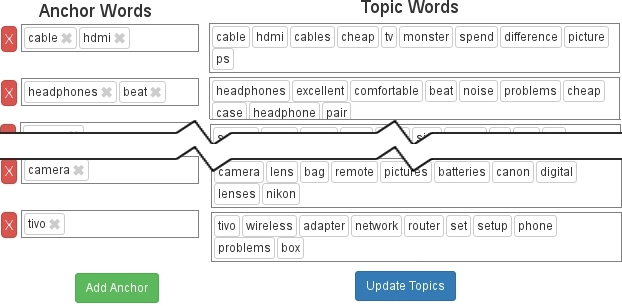
\includegraphics[width=.6\linewidth]{\filename{figures/tbuie}}
\caption{Interface for user study with multiword anchors applied to
interactive topic modeling.}
\label{fig:tbuie}
\end{figure*}

\section{Interactive Anchor Words}
\label{sec:interactive-experiments}

Given high quality anchor facets, the tandem anchor
algorithm can produce high quality topic models (particularly when the
harmonic mean combiner is used).
Moreover, the tandem anchor algorithm is fast enough to be interactive (as
opposed to model-based approaches such as the Interactive Topic Model).
We now turn our attention to our main experiment:
tandem anchors applied to the problem of interactive topic modeling.
We compare both single word and tandem anchors in our study.
We do not include the Interactive Topic Model or Utopian, as
their run times are too slow for our users.

\subsection{Interface and User Study}

To show that interactive tandem anchor words are fast, effective, and
intuitive, we ask users to understand a dataset using the anchor word
algorithm.
For this user study, we recruit twenty participants drawn from a university
student body.
The student median age is twenty-two.
Seven are female, and thirteen are male.
None of the students had any prior familiarity with topic
modeling or the \twentynews{} dataset.

Each participant sees a simple user interface
(Figure~\ref{fig:tbuie}) with topic given as a row with two columns.
The left column allows users to view and edit topics' anchor words;
the right column lists the most probable words in each
topic.\footnote{While we use topics generated using harmonic mean for
  our final analysis, users were shown topics generated using
  the min combiner.  However, this does not change our result.}
The user can remove an anchor word or drag words from the topic word lists
(right column) to become an anchor word.
Users can also add additional topics by clicking the ``Add Anchor'' to create
additional anchors.
If the user wants to add a word to a tandem anchor set that does not
appear in the interface, they manually type the word (restricted
to the model's vocabulary).
When the user wants to see the updated topics for their newly refined
anchors, they click ``Update Topics''.

We give each a participant a high level overview of topic modeling.
We also describe common problems with topic models including intruding topic
words, duplicate topics, and ambiguous topics.
Users are instructed to use their best judgement to determine
if topics are useful.
The task is to edit the anchor words to improve
the topics.
We asked that users spend at least twenty minutes, but no more than thirty
minutes.
We repeat the task twice: once with tandem anchors,
and once with single word anchors.\footnote{The order users complete these tasks is counter-balanced.}

\begin{figure*}[t!]
\centering
\includegraphics[height=.9\linewidth,angle=90]{\filename{auto_fig/user_acc}}
\caption{Classification accuracy and coherence using topic features gleaned from
user provided multiword and single word anchors. Grahm-Schmidt anchors are
provided as a baseline. For all metrics except \abr{vi}, higher is better.
Except for coherence, multiword anchors are best.}
\label{fig:user-accuracy}
\end{figure*}

\begin{figure*}[t!]
\centering
\includegraphics[height=.9\linewidth,angle=90]{\filename{auto_fig/significance}}
\caption{Topic significance for both single word and
multiword anchors. In all cases higher is better. Multiword anchors produce
topics which are more significant than single word anchors.}
\label{fig:user-significance}
\end{figure*}


\subsection{Quantitative Results}

We now validate our main result that for interactive topic modeling, tandem
anchors yields better topics than single word anchors.
Like our title-based experiments in Section~\ref{sec:oraclular-experiments},
topics generated from users become features to train and test a classifier for
the \twentynews{} dataset.
We choose this dataset for easier comparison with the Interactive Topic
Modeling result of~\newcite{hu-14:itm}.
Basedsie on our results with title-based anchors, we use the harmonic mean
combiner in our analysis.
As before, we report not only accuracy, but also multiple
clustering metrics using the confusion matrix from the classification task.
Finally, we report topic coherence.

Figure~\ref{fig:user-accuracy} summarizes
the results of our quantitative evaluation.
While we only compare user generated anchors in our
analysis, we include the unsupervised Gram-Schmidt anchors as a baseline.
Some of the data violate assumptions of normality.
Therefore, we use Wilcoxon's signed-rank test~\cite{wilcoxon-test} to determine
if the differences between multiword anchors and single word anchors are
significant.

Topics from user multiword anchors yield higher
classification accuracy (Figure~\ref{fig:user-accuracy}).
Not only is our approach more scalable than the Interactive Topic Model, but we
also achieve higher classification accuracy than~\newcite{hu-14:itm}.\footnote{However, the values are not strictly comparable, as \newcite{hu-14:itm} use
the standard chronological test/train fold, and we use random splits.}
Tandem anchors also improve clustering
metrics.\statsiguser{}

While user selected tandem anchors produce better classification features than
single word anchors,
users selected single word anchors produce topics with similar topic
coherence scores.\footnote{The difference between coherence
scores was \emph{not} statistically significant using Wilcoxon's signed-rank
test.}


To understand this phenomenon, we use quality metrics~\cite{junk-topic} for
ranking topics by their correspondence to genuine themes in the data.
Significant topics are likely skewed toward a few related words, so
we measure the distance of each topic-word distribution from the {\bf uniform}
distribution over words.
Topics which are close to the underlying word distribution of the entire data
are likely to be {\bf vacuous}, so we also measure the distance of each topic-word
distribution from the underlying word distribution.
Finally, {\bf background} topics are likely to appear in a wide range of documents,
while meaningful topics will appear in a smaller subset of the data.

Figure~\ref{fig:user-significance} reports our topic significance findings.
For all three significance metrics, multiword anchors produce more significant
topics than single word anchors.\statsiguser{}
~Topic coherence is based solely on the top $n$ words of a topic, while both
accuracy and topic significance depend on the entire topic-word distributions.
With single word anchors, topics with good coherence may still be too general.
Tandem anchors enables users to produce topics with more specific word distributions which
are better features for classification.

\begin{table*}[t!]
\begin{center}
\small
\begin{tabular}{p{.20\textwidth} p{.45\textwidth}}
\hline\hline
\bf Anchor & \bf Top Words in Topic\\\hline
\hline\multicolumn{2}{l}{\bf Automatic Gram Schmidt}\\\hline
\rowcolor{gray!35} love & love god evolution romans heard car \\
game & game games team hockey baseball heard \\
\hline\multicolumn{2}{l}{\bf Interactive Single-word}\\\hline
\rowcolor{gray!35}evolution & evolution theory science faith quote facts \\
religion & religion god government state jesus israel \\
\rowcolor{gray!35}baseball & baseball games players word teams car \\
hockey & hockey team play games season players \\
\hline\multicolumn{2}{l}{\bf Interactive Tandem}\\\hline
\rowcolor{gray!35}atheism god exists prove & god science evidence reason faith objective \\
christian jesus & jesus christian christ church bible christians \\
\rowcolor{gray!35}jew israel & israel jews jewish israeli state religion \\
baseball bat ball & hit baseball ball player games call \\
\rowcolor{gray!35}hockey nhl & team hockey player nhl win play \\
\end{tabular}
\end{center}
\caption{Comparison of topics generated for \twentynews{} using various types
of anchor words. Users combine words to create more specific
topics with tandem anchors.}
\label{tab:qual}
\end{table*}


\subsection{Qualitative Results}

We examine the qualitative differences between how users
select multiword anchor facets versus single word anchors.
Table~\ref{tab:qual} gives examples of topics generated using different
anchor strategies.
In a follow-up survey with our users, 75\% find
it easier to affect individual changes in the topics using tandem anchors
compared to single word anchors.
Users who prefer editing multiword anchors over single word anchors
often report that multiword anchors make it easier to merge similar
topics into a single focused topic by combining anchors.
For example, by combining words related to \underline{Christianity}, users create
a topic which is highly specific, and differentiated from general
religion themes which also include Atheism and Judaism.

While users find that use tandem anchors is easier, only 55\% of our users
say that they prefer the final topics produced by tandem anchors compared
to single word anchors.
This is in harmony with our quantitative measurements of topic coherence, and
may be the result of our stopping criteria: when users judged the topics to be
useful.

However, 100\% of our users feel that the topics created through interaction
were better than those generated from Gram-Schmidt anchors.
This was true regardless of whether we used tandem anchors or single word
anchors.

Our participants also produce fewer topics with multiword anchors.
The mean difference between topics under single word anchors and
multiple word anchors is $9.35$.
Follow up interviews reveal that participants resolve ambiguous topics
by creating a new anchor
for each of the ambiguous terms, thus explaining the proliferation of topics
for single word anchors.
In contrast, fixing an ambiguous tandem anchor is simple: users just add more
terms to the anchor facet.


\newpage

\section{Conclusion}
\label{sec:conclusion}

Tandem anchors extend the anchor words algorithm to allow multiple words to be
combined into anchor facets.
For interactive topic modeling, using anchor facets in place of single word
anchors produces higher quality topic models and are more intuitive to use.
Furthermore, our approach scales much better than existing interactive topic
modeling techniques, allowing interactivity on large datasets for which
interactivity was previous impossible.

In addition to a faster, interactive algorithm, anchor methods provide
a more direct path from user input to a final clustering output.By making interactivity both fast and intuitive, tandem anchors help
remove some of the mystery of machine learning algorithms, improving
trust in algorithms and eventual adoption.

\vspace{1cm}

\section*{Acknowledgements}

This work was supported by the collaborative NSF Grant IIS-1409287 (\abr{umd}) and
IIS-1409739 (\abr{byu}). Boyd-Graber is also supported by NSF grants \abr{iis}-1320538 and
\abr{ncse}-1422492.


\newpage

\small
\bibliographystyle{style/acl_natbib}
\bibliography{bib/jlund,bib/jbg}

\end{document}
